\documentclass[letterpaper,9pt,twocolumn,twoside,]{pinp}

%% Some pieces required from the pandoc template
\providecommand{\tightlist}{%
  \setlength{\itemsep}{0pt}\setlength{\parskip}{0pt}}

% Use the lineno option to display guide line numbers if required.
% Note that the use of elements such as single-column equations
% may affect the guide line number alignment.

\usepackage[T1]{fontenc}
\usepackage[utf8]{inputenc}

% pinp change: the geometry package layout settings need to be set here, not in pinp.cls
\geometry{layoutsize={0.95588\paperwidth,0.98864\paperheight},%
  layouthoffset=0.02206\paperwidth, layoutvoffset=0.00568\paperheight}

\definecolor{pinpblue}{HTML}{185FAF}  % imagecolorpicker on blue for new R logo
\definecolor{pnasbluetext}{RGB}{101,0,0} %



\title{A Template for Two or One-Column Vignettes}

\author[a]{First Author}
\author[a,b]{Second Author}

  \affil[a]{Institute of Smoke and Magic, University of Sometown, Sometown, XY,
12345}
  \affil[b]{Department of Neat Tricks, Whereever State University, Someplace, MC,
67890}

\setcounter{secnumdepth}{0}

% Please give the surname of the lead author for the running footer
\leadauthor{Author and Author}

% Keywords are not mandatory, but authors are strongly encouraged to provide them. If provided, please include two to five keywords, separated by the pipe symbol, e.g:
 \keywords{  one |  two |  optional |  keywords |  here  }  

\begin{abstract}
Your abstract will be typeset here, and used by default a visually
distinctive font. An abstract should explain to the general reader the
major contributions of the article.
\end{abstract}

\dates{This version was compiled on \today} 


% initially we use doi so keep for backwards compatibility
% new name is doi_footer
\doifooter{\url{https://cran.r-project.org/package=YourPackage}}

\pinpfootercontents{YourPackage Vignette}

\begin{document}

% Optional adjustment to line up main text (after abstract) of first page with line numbers, when using both lineno and twocolumn options.
% You should only change this length when you've finalised the article contents.
\verticaladjustment{-2pt}

\maketitle
\thispagestyle{firststyle}
\ifthenelse{\boolean{shortarticle}}{\ifthenelse{\boolean{singlecolumn}}{\abscontentformatted}{\abscontent}}{}

% If your first paragraph (i.e. with the \dropcap) contains a list environment (quote, quotation, theorem, definition, enumerate, itemize...), the line after the list may have some extra indentation. If this is the case, add \parshape=0 to the end of the list environment.

\acknow{This template package builds upon, and extends, the work of the
excellent \href{https://cran.r-project.org/package=rticles}{rticles}
package, and both packages rely on the
\href{http://www.pnas.org/site/authors/latex.xhtml}{PNAS LaTeX} macros.
Both these sources are gratefully acknowledged as this work would not
have been possible without them. Our extensions are under the same
respective licensing term
(\href{https://www.gnu.org/licenses/gpl-3.0.en.html}{GPL-3} and
\href{https://www.latex-project.org/lppl/}{LPPL (\textgreater{}= 1.3)}).}

\hypertarget{introduction}{%
\subsection{Introduction}\label{introduction}}

This \emph{pinp is not PNAS} template started when the introduction to
\href{http://dirk.eddelbuettel.com/code/rcpp.html}{Rcpp} by
\cite{PeerJ:Rcpp} was converted into this updated
\href{https://eddelbuettel.github.io/pinp/Rcpp-introduction.pdf}{Rcpp
Introduction} vignette. It is based on the
\href{https://github.com/rstudio/rticles/tree/master/inst/rmarkdown/templates/pnas_article}{pnas\_article}
template of the wonderful
\href{https://cran.r-project.org/package=rticles}{rticles} package by
\cite{CRAN:rticles}. The conversion from markdown to latex is
facilitated by
\href{https://cran.r-project.org/package=rmarkdown}{rmarkdown}
\citep{CRAN:rmarkdown} and
\href{https://cran.r-project.org/package=knitr}{knitr}
\citep{CRAN:knitr}. The underlying LaTeX macros are from
\href{http://www.pnas.org/site/authors/latex.xhtml}{pnas.org}.

The remainder of the document carries over from the corresponding
\href{https://github.com/rstudio/rticles/tree/master/inst/rmarkdown/templates/pnas_article}{pnas\_article}
template document. but has been edited and updated to our use case. A
few specific tips follow. In general, for fine-tuning some knowledge of
LaTeX is helpful.

\hypertarget{author-affiliations}{%
\subsection{Author Affiliations}\label{author-affiliations}}

Per common academic best practice, you can include your department,
institution, and complete address, with the ZIP/postal code, for each
author. Use lower case letters to match authors with institutions, as
shown in the example. Authors with an ORCID ID may supply this
information at submission.

\hypertarget{document-options}{%
\subsection{Document Options}\label{document-options}}

We support several options via the YAML header

\begin{itemize}
\tightlist
\item
  Setting a DOI or URL footer, for example for the CRAN package URL,
  which is placed in the bottom-left footer of the title page and even
  pages;
\item
  Setting a footer label, for example \emph{YourPackage Vignette}
  stating your package, which is placed in the bottom-right footer on
  odd pages;
\item
  Setting a free-form author field used on the inside footer;
\item
  Optional \emph{Draft} watermark to be added to each page;
\item
  Line of custom text in subtitle (\texttt{date\_subtitle}) suitable to
  give publication info of the draft, e.g.~journal name in a post-print;
\item
  Document date that appears in the footer can be specified manually
  using \texttt{document\_date}.
\end{itemize}

\hypertarget{references}{%
\subsection{References}\label{references}}

Here we differ from PNAS and suggest natbib. References will appear in
author-year form. Use \texttt{\textbackslash{}citet\{\}},
\texttt{\textbackslash{}citep\{\}}, etc as usual.

We default to the \texttt{jss.bst} style. To switch to a different
bibliography style, please use \texttt{biblio-style:\ style} in the YAML
header.

\hypertarget{inline-r-code}{%
\subsection{Inline R Code}\label{inline-r-code}}

The PNAS sample included a fixed PNG image here, but this document
prefers to show the results and embedding of \emph{R} code.

\begin{Shaded}
\begin{Highlighting}[]
\KeywordTok{library}\NormalTok{(ggplot2)}
\KeywordTok{ggplot}\NormalTok{(mtcars, }\KeywordTok{aes}\NormalTok{(wt, mpg)) }\OperatorTok{+}
\StringTok{    }\KeywordTok{geom_point}\NormalTok{(}\DataTypeTok{size=}\DecValTok{3}\NormalTok{, }\KeywordTok{aes}\NormalTok{(}\DataTypeTok{colour=}\KeywordTok{factor}\NormalTok{(cyl))) }\OperatorTok{+}
\StringTok{    }\KeywordTok{theme}\NormalTok{(}\DataTypeTok{legend.position=}\StringTok{"none"}\NormalTok{)}
\end{Highlighting}
\end{Shaded}

\begin{figure}

{\centering 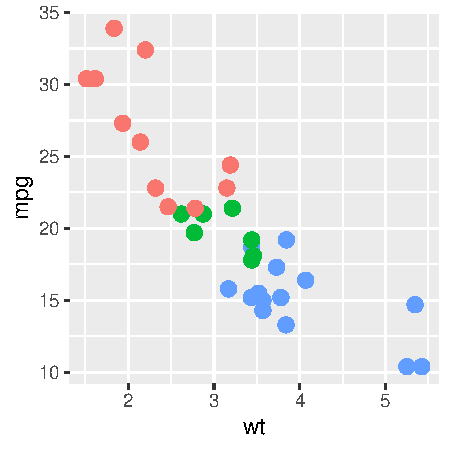
\includegraphics{ExecSum_files/figure-latex/figex-1} 

}

\caption{Narrow ggplot2 figure}\label{fig:figex}
\end{figure}

Here we use a standard knitr bloc with explicit options for

\begin{itemize}
\tightlist
\item
  figure width and height (\texttt{fig.width}, \texttt{fig.height}),
  both set to three inches;
\item
  whether the code is shown (\texttt{echo=TRUE}); and
\item
  the caption (\texttt{fig.cap}) as shown above.
\end{itemize}

\hypertarget{digital-figures}{%
\subsection{Digital Figures}\label{digital-figures}}

Markdown, Pandoc and LaTeX support \texttt{.eps} and \texttt{.pdf}
files.

Figures and Tables should be labelled and referenced in the standard way
using the \texttt{\textbackslash{}label\{\}} and
\texttt{\textbackslash{}ref\{\}} commands.

The R examples above show how to insert a column-wide figure. To insert
a figure wider than one column, please use the
\texttt{\textbackslash{}begin\{figure*\}...\textbackslash{}end\{figure*\}}
environment.

One (roundabout) way of doing this is to \emph{not} actually plot a
figure, but to save it in a file as the following segment shows:

\begin{Shaded}
\begin{Highlighting}[]
\KeywordTok{library}\NormalTok{(ggplot2)}
\NormalTok{p <-}\StringTok{ }\KeywordTok{ggplot}\NormalTok{(}\DataTypeTok{data =}\NormalTok{ midwest,}
            \DataTypeTok{mapping =} \KeywordTok{aes}\NormalTok{(}\DataTypeTok{x =}\NormalTok{ area,}
                          \DataTypeTok{fill =}\NormalTok{ state,}
                          \DataTypeTok{color =}\NormalTok{ state)) }\OperatorTok{+}
\StringTok{    }\KeywordTok{geom_density}\NormalTok{(}\DataTypeTok{alpha =} \FloatTok{0.3}\NormalTok{)}
\CommentTok{## save to file}
\KeywordTok{suppressMessages}\NormalTok{(}\KeywordTok{ggsave}\NormalTok{(}\StringTok{"densities.pdf"}\NormalTok{, p))}
\end{Highlighting}
\end{Shaded}

This file is then included via standard LaTeX commands.

\begin{figure*}
  \begin{center}
    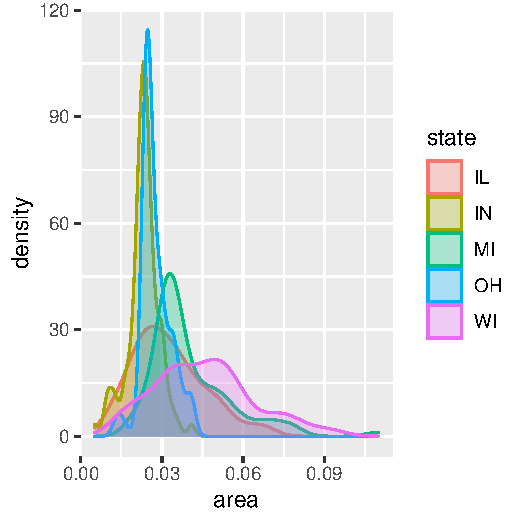
\includegraphics[width=0.66\textwidth, height=3.5in]{densities} 
  \end{center}
  \caption{Wide ggplot2 figure}\label{fig}
\end{figure*}

\hypertarget{typeset-code-but-do-not-run-it}{%
\subsection{Typeset Code (But Do Not Run
It)}\label{typeset-code-but-do-not-run-it}}

We can also just show code.

\begin{Shaded}
\begin{Highlighting}[]
\NormalTok{xx <-}\StringTok{ }\NormalTok{faithful[,}\StringTok{"eruptions"}\NormalTok{]}
\NormalTok{fit <-}\StringTok{ }\KeywordTok{density}\NormalTok{(xx)}
\KeywordTok{plot}\NormalTok{(fit)}
\end{Highlighting}
\end{Shaded}

This simply used a pandoc bloc started and ended by three backticks,
with \texttt{r} as the language choice. Similarly, \emph{many} other
languages can be typeset directly simply by relying on pandoc.

\hypertarget{single-column-equations}{%
\subsection{Single column equations}\label{single-column-equations}}

Authors may use 1- or 2-column equations in their article, according to
their preference.

To allow an equation to span both columns, options are to use the
\texttt{\textbackslash{}begin\{figure*\}...\textbackslash{}end\{figure*\}}
environment mentioned above for figures. The
\texttt{\textbackslash{}begin\{widetext\}...\textbackslash{}end\{widetext\}}
environment as shown in equation \ref{eqn:example} below is deprecated,
but \LaTeX commands \texttt{\textbackslash{}onecolumn} and
\texttt{\textbackslash{}twocolumn} work fine.

Please note that this option may run into problems with floats and
footnotes, as mentioned in the \href{http://texdoc.net/pkg/cuted}{cuted
package documentation}. In the case of problems with footnotes, it may
be possible to correct the situation using commands
\texttt{\textbackslash{}footnotemark} and
\texttt{\textbackslash{}footnotetext}.

\begin{equation}
  \begin{aligned}
(x+y)^3&=(x+y)(x+y)^2\\
       &=(x+y)(x^2+2xy+y^2) \\
       &=x^3+3x^2y+3xy^3+x^3. 
       \label{eqn:example} 
  \end{aligned}
\end{equation}

%\showmatmethods
\showacknow


\bibliography{pinp}
\bibliographystyle{jss}



\end{document}

